\documentclass[11pt]{amsart}
\usepackage{geometry}                % See geometry.pdf to learn the layout options. There are lots.
\geometry{letterpaper}                   % ... or a4paper or a5paper or ... 
%\geometry{landscape}                % Activate for for rotated page geometry
%\usepackage[parfill]{parskip}    % Activate to begin paragraphs with an empty line rather than an indent
\usepackage{graphicx}
\usepackage{amssymb}
\usepackage{epstopdf}
\usepackage{fullpage}
\DeclareGraphicsRule{.tif}{png}{.png}{`convert #1 `dirname #1`/`basename #1 .tif`.png}

\newtheorem{Def}{Definition} %[section]
\newtheorem{Example}[Def]{Example}
\newtheorem{Prop}[Def]{Property}
\newtheorem{Lemma}[Def]{Lemma}
\newtheorem{Thm}[Def]{Theorem}
\newtheorem{Conj}[Def]{Conjecture}
\newtheorem{Cor}[Def]{Corollary}
\newtheorem{Question}[Def]{Question}
\newtheorem{Answer}[Def]{Answer}

\newcommand\bpf[1][]{\smallskip\noindent{\bf Proof#1.}\quad}
\newcommand\epf{\qed\medskip}
\newcommand{\up}[1]{\ensuremath{^{\textrm{#1}}}}

\newcommand\N{\mathbb N}
\newcommand\fin{\mathrm{fin}}

\title{Brief Article}
\author{The Author}
%\date{}                                           % Activate to display a given date or no date

\begin{document}

{\bf Ideas While Learning Set Theory} \hfill Tyler Neylon

\medskip

These notes are not meant to be considered an academic paper,
or anything close to that. They are a collection of my personal
thoughts while learning set theory.

\section{Equivalences}

This section describes some explicitly constructed, somewhat natural 1-1 correspondences between
some collections of objects, such as sets, multi sets, lists, trees, and $\N$.

\subsection{Numbers $\leftrightarrow$ binary trees}

Choose any 1-1 correspondence $f : \N_{\ge 1} \to \N^2_{\ge 0}$.
I like to think of such a map as a counting of grid points in an array, such as this:

$$
\begin{array}{c|cccc}
 & 0 & 1 & 2 & 3 \\
 \hline
 0 & 1 & 2 & 4 & 7 \\
 1 & 3 & 5 & 8 \\
 2 & 6 & 9 \\
 3 & 10 &&& \ddots \\
\end{array}
$$

That's what Hausdorff calls ``the diagonal array.''
It's pretty easy to compute both ways.

Once you have $f = (f_1, f_2)$, then you build a binary
tree from a number $n$ recursively like this:

If $n=0$, then it's the empty tree (no root).
Otherwise, give it the left child $f_1(n)$ and
right child $f_2(n)$, keeping in mind that if
either has value 0, this means no child in that direction.
If you don't want to count the no-root tree, then start
counting at $n=1$ instead of $n=0$.

\subsection{Numbers $\leftrightarrow$ ordered $n-$ary trees}

An ordered $n-$ary tree is the natural extension of binary trees.
To be clear, binary trees are used (in my experience) most often
in a computer science context, where the left and right subtrees
are always distinguished - i.e., they are ordered. This is a bit
different from the typical math tree, where there is no intrinsic order.

The mapping is exactly the same as the binary case, except that
we must choose a 1-1 correspondence $g: \N_{\ge 1} \to \N^n_{\ge 0}$;
then the $k^\text{th}$ child of a tree numbered by $m$ will be
numbered by $g_k(m)$, where $g_k(m)$ is the  $k^\text{th}$ coordinate
of $g(m)$.

Keep in mind that this scheme allows for any number of children
between 0 and $n$, inclusively, as 0 values indicate the lack of a child
in a given position.

\subsection{Numbers $\leftrightarrow$ unordered $n$-ary trees}

This is the same as the ordered case, except that the $k$\up{th} child
of a tree numbered by $m$ is given by $\sum_{\ell \le m} g_\ell(m)$,
where again $g_\ell(m)$ is the $\ell$\up{th} coordinate of $g(m)$.

By using the cumulative sum of the coordinates, we eliminate duplicate
trees that have the same $g_\ell(m)$ vector except for order of coordinates.
I think of this equivalence more directly by going in the reverse direction.
Given a set of subtrees, take the index of all of them, and treat that as a list
of nonnegative integers. Sort these, and take their differences. The result
is a unique vector of nonnegative integers that forms the $g_\ell(m)$ vector.

\subsection{Numbers $\leftrightarrow$ unordered, duplicate-free, any-arity trees $\leftrightarrow$ sets}

This is conceptually similar to the last case, except that we
disallow any equal children, and a node may have any finite number of children.

Choose an onto function
$$ g : \N_{\ge 1} \to \bigcup_{k \ge 0} \N_{\ge 1}^k,$$
where we treat $\N_{\ge 1}^0$ as a singleton containing a zero-length vector.
I find it helpful to think of $f(1)$ as mapping to the zero-length vector.

In this enumeration, we skip over the empty tree completely, and
the tree numbered by $m$ has children given by $g(m)$, where
the $k$\up{th} child is numbered by $\sum_{\ell \le k} g_\ell(m)$.
Because each coordinate is positive, no two numbers in the cumulative
sum may be equal, so that duplicates are avoided. As in the last
case, there is also only one ordering (sorted by number) for each list
of children. That completes the equivalence between numbers and
unordered, duplicate-free, any-arity trees.

Now let's take such a tree, and turn it into a set, in a way that works as
a bijection. The tree with a single node maps to the empty set.
Any tree with $n$ children maps to a set with $n$ elements, each element
corresponding to a child of the tree. That completely describes the
mapping.

Below are some tree $\leftrightarrow$ set examples, where I use the von Neumann numbering
system with $n = \{0, 1, \ldots, n-1\}$ to help describe the sets.

\centerline{
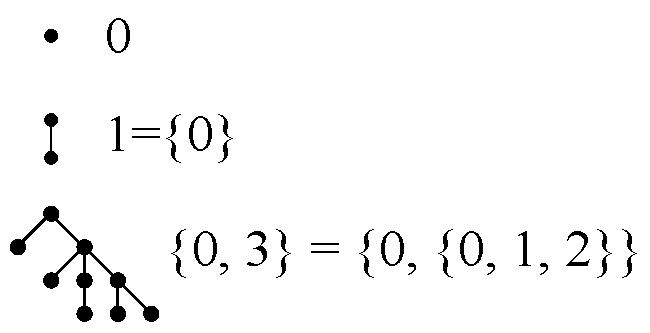
\includegraphics[width=6.0cm]{set_theory_ideas2.pdf}
}

\subsection{Multisets $\leftrightarrow$ unordered, any-ary trees}

This one is easy. Each child of a node is a member of the multiset.
That's all that is needed. So the empty set $\{\}=0$ is a single node, and
a tree with one root and one child total is the set $\{0\}$.
This is basically the same as the last case except that we both allow
duplicates in the tree and in the ``sets'' which then become multisets.

I like this equivalence because such trees are essentially the same
(single-component) trees that are already studied in graph theory,
having a special designated root node. I'm particularly curious about
the similarity relation given by saying that multisets $m_1$ and $m_2$
are similar iff they share the same tree (with different roots, possibly).
For example, $\{0, 0, 0\} \sim \{\{0, 0\}\}$ since they are both multisets
given by the tree with one central node adjacent to three other nodes,
each of which is otherwise isolated (like the letter Y).

I've noticed that in this equivalence,
$$ \#(\text{tree edges}) = \#(\text{sibling relationships}) + \#(\text{child relationships}), $$
where the number of sibling relationships is the number of commas in writing out
the multiset, and the number of child relationships is the number of open braces $\{$ in
writing it out, assuming that all empty sets are written as $0$.
This characteristic of a multiset (\# siblings + \# children) cannot change within
a similarity set.

\subsection{Binary trees $\leftrightarrow$ pairs}

Binary trees are usually considered as rooted connected finite trees where each
node has 0, 1, or 2 ordered children. Such a tree is a fundamental structure in
computer science.

For this one equivalence, I will restrict attention to binary trees where each
node has either 0 or 2 children --- having exactly 1 child is not allowed.

By a {\em pair}, I mean an ordered pair of two elements, in the sense that
these could replace sets as the fundamental unit of an axiomitization of math,
much as multisets, or lists could.

This equivalence is very intuitive. The left child is the left element of the pair,
and the right child is the right element.

Can we do something similar with binary trees that also allow for exactly one child,
either left or right? This would exactly match a very common interpretation of
``binary tree'' in other studies, and that's what we do in the next equivalence.

\subsection{Binary trees $\leftrightarrow$ lists}

A {\em list} is a finite ordered multiset of elements. (I can imagine lists which
do not need to be finite, such as being indexed by ordinals, but for now I'll
just talk about finite lists.)
I'll write the list with elements $a_1, a_2, \ldots, a_k$ as
$$(a_1, a_2, \ldots, a_k).$$
Not a big surprise there, but I will use this notation below to help clarify
this equivalence.

The idea for this equivalence is to treat each left-child relationship in the tree as an
element-of relationship in the list, and each right-child in the tree as a sibling in the list.
The empty list $() = 0$ is represented by the empty tree, with zero nodes.

Some examples might help to clarify the idea.

\centerline{
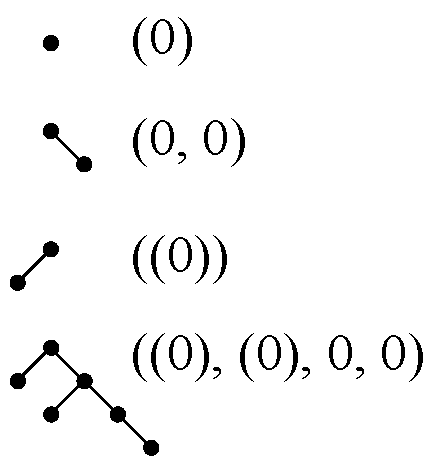
\includegraphics[width=4.0cm]{set_theory_ideas3.pdf}
}

Here is another perspective of this equivalence: we will turn a tree
into a list by doing a depth-first, left-first traversal of a tree, and turn
that into a list. If the tree is empty, write \fbox{$0$} and you're done.
Otherwise, write an open parenthesis \fbox{$($}, and begin.
Each time you go to a left child, write \fbox{$($}. When you're at a node without a left child,
write \fbox{$0$}. When you backtrack up from a left child, write a \fbox{$)$}.
When you go to a right child, write a comma \fbox{$,\phantom|$} .
Finally add a single \fbox{$)$} at the end once you're done with
the whole tree.

\section{Total Orders}

\subsection{A fixed-point theorem for total orders}

The following result was motivated originally by the
Banach fixed-point theorem. After proving it, I found out
about the Bourbaki-Witt (B-W) theorem, which is extremely similar,
and probably only this theorem or B-W is needed (i.e. one can be
derived easily from the other), although I haven't figured out which yet.

The notation $\sup (A)$ means $\min \{x : x \ge a \forall a \in A\}$,
which does not exist for every set $A$.

\begin{Thm}
Suppose that $X$ is totally ordered, that $\sup (A)$ exists
$\forall \text{ nonempty } A\subset X$ with an upper bound,
and that $f:X\to X$ is an
order-preserving map with $x_0 < f(x_0)$ and $f(x_1) < x_1$,
for $x_0 < x_1$. Then $\exists y \in (x_0, x_1)$ with $f(y) = y$.
\end{Thm}

\bpf
Define
$$ A = \{ y \in [x_0, x_1] : x_0 \le z \le y \implies f(z) > z \}. $$
Intuitively, $A$ is the largest convex set with left endpoint $x_0$
where $f(a) > a \forall a \in A$.

% insert set_theory_ideas1.pdf here

\centerline{
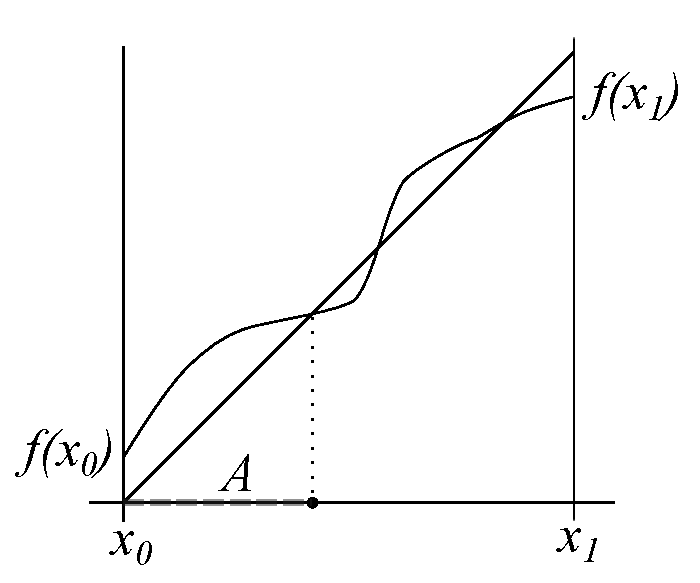
\includegraphics[width=6.0cm]{set_theory_ideas1.pdf}
}

Let $\beta = \sup (A)$, which exists since $A$ is nonempty,
having $x_0 \in A$, and has an upper bound, $x_1$.

If $\gamma = f(\beta) < \beta$, then $\gamma \in A$, but
$$ \gamma < \beta \implies f(\gamma) < f(\beta)
  \implies f(\gamma) < \gamma, $$
%$f(\gamma) = f(f(\beta)) < f(\beta) = \gamma$,
which contradicts
$f(\gamma) > \gamma$ for everything in $A$.
So $f(\beta) \ge \beta$. If $f(\beta) = \beta$, we're done,
so assume $f(\beta) > \beta$.

Suppose $w \in [x_0, x_1]$.

If $\beta < w$ and $\big(f(b) > b \,\forall\, b \in (\beta, w]\big)$,
then $w \in A$, which would contradict $w > \beta \ge A$.
So $\exists\, b_0$ with $\beta < b_0 \le w$
and $f(b_0) \le b_0$.  Then $f(\beta) < f(b_0) \le b_0 \le w$.

At this point we have both
$$ \beta < w \implies f(\beta) < w $$
and
$$ \beta > w \implies w \in A \implies f(\beta) > f(w) > w.$$

So $f(\beta) \in [x_0, x_1] \setminus \{ < \beta \} \setminus \{ > \beta \} = \{\beta\}$.
\epf

Note that $\sup (A)$ need only  exist for the specific set $A$
used in the proof, so that part of the theorem's conditions could be relaxed.

\subsection{Matching well orders}

This is an old idea for me, but I wanted to record it in this section.

First, we need a lemma from Jech's {\em Set Theory} (I have the 3\up{rd} edition).

\begin{Lemma}\label{b_squared_is_b_lemma}
Suppose infinite ordinal $\omega_a$ is the first  of its cardinality -- that is, $|\omega_b| < |\omega_a|$
for all $\omega_b < \omega_a$.
Also suppose that well-ordered set $A$ is of order type $\omega_a$. Then any
proper subset $B \subsetneq A$ has $|B|^2 = |B| < |A|$.
\end{Lemma}

The fact that $A$ can be well-ordered as $\omega_a$ is not necessarily true without
the axiom of choice (not obvious), and in fact someone (I think Tarski) has proven that
if $|A|^2=|A|$ for all infinite sets $A$, then the axiom of choice must hold.

(Asaf Karagila helped me out a bit here via math.stackexchange.com.)

Theorem 3.5 in Jech has a proof which also proves this lemma.

There is an interesting perspective on this lemma which I particularly like:

\begin{Lemma}
Suppose infinite ordinal $\omega_a$ is the first  of its cardinality, and its
cardinality is not the limit of $|\omega_b|$ for $\omega_b < \omega_a$.
Then any increasing ordinal sequence $\left< \eta_i | i \in \omega_b \right>$
with $\eta_i, \omega_b < \omega_a$ must have $\lim_i \eta_i < \omega_a$.
\end{Lemma}

The lemma follows because all the $\eta_i$ must have $|\eta_i| \le \mathfrak b$,
where $\mathfrak b$ is the largest cardinal in $\omega_a$ (which means
$\mathfrak b < |\omega_a|$).
We also know that $|\omega_b| \le \mathfrak b$,
and by the previous lemma, that $\mathfrak b^2 = \mathfrak b$. So
$$ | \lim \eta_i | = | \cup_{i\in\omega_b} \eta_i | \le \mathfrak b^2 = \mathfrak b < |\omega_a|.$$

I'd summarize that last lemma as ``you can't sneak up on successor ordinals.''

Here's the result these lemmas are used for:

\begin{Thm}[Matching Well Orders]
Suppose infinite set $X$ is well ordered by both $\le_1$ and $\le_2$.
Then there is a subset $Y \subset X$ with $|Y| = |X|$ on which
$\le_1$ and $\le_2$ agree; the axiom of choice is not needed.
\end{Thm}

The proof in the general form looks a bit unintuitive, so first I'll mention the
main idea by looking at a special case with $X=\N$.
Suppose I have two orders $\le_1$ and $\le_2$ such that
$\N$ under $\le_i$ has order type $\omega$ for both $i=1,2$.

For each integer $n$, we'll inductively build a subset of $\N$ on which
these orders agree. For the base case, we can just use the $\le_1$-min
element.

Suppose we have set $S\subset\N$ on which the orders agree.
The next element $e$ that we append must have both $S <_1 e$ and $S <_2 e$.
So we want to exclude $T = \{ m : m \le_2 s \text{ for any } s \in S\}$.
Because $\N$ under $\le_2$ has order type $\omega$, we know that each
set $\{ \le_2 s \}$ is finite; $T$ is the union of $\{ \le_2 s\}$ over $s\in S$, so that
$T$ is also finite. Thus $U = \N - S - T$ is nonempty, and we can choose the
$\le_1$-min element of $U$ as the next element to append to $S$.

By induction on the size of $S$, we get a countably infinite subset of $\N$ on which the orders agree.
I don't think it's obvious how to extend this to an arbitrary set $X$, so I'll prove that carefully.

I would summarize this special case as saying, if you have any two enumerations of $\N$, there's
an infinite subset on which they are identical.

For the proof I will also use this easy lemma:

\begin{Lemma}\label{first_ordinal_lemma}
If $X$ is well ordered by $\le$, then there is a subset $Y\subset X$ with
$|Y| = |X|$ where the order type of $Y$ under $\le$ is the first ordinal
with cardinality $|X|$.
\end{Lemma}

This lemma is true because we can look at the set $Z = \{ x\in X : |\{ < x \}| = |X| \}$.
If $Z$ is empty, then $Y=X$ satisfies the lemma. Otherwise, $Z$ has a $\le$-first element $z$,
and we can let $Y = \{ < z \}$.

\bpf
Ok, let's get this party started.

We have an infinite set $X$ that is well ordered by $\le_1$ and $\le_2$.
Let $\omega_x$ denote the first ordinal number with the cardinality of $X$.

We'll split this into two cases:

{\bf Case 1 } $|\omega_x|$ is a successor cardinal

When we say {\em successor cardinal}, we mean among
the cardinals that derive from ordinals. These cardinals are
well ordered, so they are either successors or limits, without
need for the axiom of choice. Hence our split into cases 1 and 2 ---
$|\omega_x|$ is a successor or limit cardinal --- is valid without the axiom of choice.

Use lemma \ref{first_ordinal_lemma} on both $\le_1$ and $\le_2$ (one
at a time) to get a subset $Y \subset X$
with $|Y| = |X|$ where $|\{ <_i y \}| < |X|$ for all $y\in Y$, $i=1,2$.

We will now define, via transfinite induction, a subset of $Y$ on which the orders agree.
We'll use a 1-1 function $f : \omega_x \to Y$, defining $f(\chi)$ in terms
of $f( \{ < \chi \} )$, so that the orders agree on $f( \{ \le \chi \} )$.

Suppose $f$ is already defined on the domain $\{ < \chi \}$ for some fixed $\chi \in \omega_x$.
Let $S = f( \{ < \chi \} )$, and 
let $T = \{ y \in Y : y \le_2 s \text{ for some } s \in S \}$.
This way, any element $e \in Y - T$ must have $e >_2 s$ for every $s \in S$.

Because $|\omega_x|$ is a successor cardinal, it has an immediate predecessor
$\mathfrak b$.
We chose $Y$ so that $|\{\le_2 s\}| < |Y|=|X|$, so $|\{\le_2 s\}| \le \mathfrak b$.
And $|S| = |\{ < \chi \}| < |\omega_x| = |X|$, so $|S| \le \mathfrak b$.
Then $|T| = |\cup_{s\in S}\{\le_2 s\}| \le \mathfrak b^2 = \mathfrak b < |Y|$,
so that $Y-T$ is nonempty
(the $\mathfrak b^2 = \mathfrak b$ part comes from lemma \ref{b_squared_is_b_lemma}).
Thus we can define $f(\chi )$ as the
$\le_1$-first element of $Y-T$, completing case 1.

{\bf Case 2 } $|\omega_x|$ is a limit cardinal

In this case, we can build $f_\mathfrak b$ for any ordinal-based cardinal $\mathfrak b$ below
$|\omega_x|$ using the technique from case 1. If each step results in a
superset of the previous steps, then we can take the union of the results to
get a consistent subset of $Y$ with the same cardinality.

Let's build $f_\alpha$ to have cardinality $\aleph_\alpha$.
In particular, let $\omega_\alpha$ be the first ordinal so that
$|\omega_\alpha| = \aleph_\alpha$, and we'll define
$f_\alpha$ on the domain $\omega_\alpha$.

{\bf Case 2a} $\aleph_\alpha$ is a successor cardinal

(Again the term successor cardinal in this proof means among
ordinal-based cardinals, to avoid using the axiom of choice.)

Let $\aleph_\beta$ denote the predecessor of $\aleph_\alpha$,
with $\omega_\beta$ the first ordinal of size $\aleph_\beta$.
Then $f$ has already been defined on $\omega_\beta$.

Choose $Y' \subset X$ so that $Y'$ has order type $\omega_\alpha$
under $\le_1$. Choose $Y\subset Y'$ so that $|Y| = |Y'| = \aleph_\alpha$
and $| \{ <_2 y \} | \le \aleph_\beta$ using lemma \ref{first_ordinal_lemma}.
Note that this $Y$ is a superset of any other $Y$ chosen for a smaller cardinal
as $\aleph_\alpha$.

We'll inductively define $f_\alpha$ on every $\chi \in \omega_\alpha$ with $\chi \ge \omega_\beta$.
For $\chi \in \omega_\beta$, we set $f_\alpha(\chi) = f_\beta(\chi)$.

As above, let $S = f_\alpha( \{ < \chi \} )$,
and $ T = \{ y \in Y : y \le_2 s \text{ for some } s \in S \}$; we'll verify that the size of $T$ is bounded.
We know $|S| = \aleph_\beta$ and $|\{ \le_2 s \} | \le \aleph_\beta$, so
$$ |T| = \left|\cup_{s\in S} \{ \le_2 s \}\right| \le \aleph_\beta^2 = \aleph_\beta < |Y| = \aleph_\alpha. $$

This means $Y-T$ is nonempty, and we can define $f_\alpha(\chi)$ as its $\le_1$-first element, as before.

{\bf Case 2b} $\aleph_\alpha$ is a limit cardinal

We have been careful to define $f_\alpha$ consistently on all previous sets ---
in other words, if $\chi$ is in the domain of $f_\gamma$ for any $\aleph_\gamma < \aleph_\alpha$,
then $\chi$ is in the domain of $f_\alpha$ and $f_\gamma(\chi) = f_\alpha(\chi)$.

Thinking of $f_\gamma$ as a set of ordered pairs,
we can use a union to define a limit:
$$ f_\alpha = \cup_{\aleph_\gamma < \aleph_\alpha} f_\gamma. $$

If there exists $x, y$ in the range of $f_\alpha$ such that $x <_1 y <_2 x$ or $x <_2 y <_1 x$, then
there must be some first cardinal $\aleph_\gamma < \aleph_\alpha$ for which both $x$ and $y$ are in the
range of $f_\gamma$. But then $f_\gamma$ would itself have provided a set (as its range)
on which the orders do not agree, which is impossible.

Therefore the orders still agree on the range of $f_\alpha$.

The induction holds until, and including the case where, we get to the cardinality $\aleph_\alpha = |X|$,
at which point the theorem is proven.
\epf

After just finishing up that proof, I realize it is not nearly as concise as it could be.
Basically everything we need is included in case 2. I could try to clean it up later.

\section{Ordinal Numbers}

\subsection{Left addition and multiplication}

In \S 14 of Hausdorff, he points out that
$$ \alpha < \beta \implies \alpha + \mu \le \beta + \mu,$$
$$ \alpha < \beta \implies \alpha \mu \le \beta \mu.$$

Which led me to ask

\begin{Question}
When is true that $\alpha < \beta$, but either
$\alpha + \mu = \beta + \mu$, or $\alpha\mu = \beta\mu$ ?
\label{q1}
\end{Question}

This is interesting because it can be used for right cancellation.
If some conditions on $\alpha, \beta, \mu$ indicate that
\begin{equation}
\alpha\mu = \beta\mu \implies \alpha = \beta,
\label{eqn1}
\end{equation}
 then we can effectively
perform something like division by $\mu$ on the right; similar
reasoning in the additive version can be used for something like subtraction on the right.
Because (\ref{eqn1}) is not always true, we do not always have this
division-on-the-right.

In retrospect, this question is also interesting because exploring it lead me to
better understand ordinal structures, such as having a stronger sense of
what kind of distribution we can do on the left --- that is, addressing 

\begin{Question}
We know that $\gamma(\alpha + \beta) = \gamma\alpha + \gamma\beta$,
which is distribution on the right.
How can we similarly expand the expression $(\alpha + \beta)\gamma$,
which is distribution on the left?
\label{q2}
\end{Question}

The first result is that, when $\alpha < \beta$, $\gamma > 0$:
\begin{equation}
\begin{cases}
\gamma + \mu = \mu  & \text{ iff } \quad \mu \ge \gamma\omega \\
\alpha + \mu = \beta + \mu & \text{ iff } \quad \mu \ge (-\alpha + \beta)\omega 
\end{cases}
\label{eqn2}
\end{equation}

Let's verify that. Write $\mu = \gamma\eta + \xi$ (as per (3) on p. 74 in Hausdorff,
division among ordinals). Then
$\gamma + \mu = \gamma + \gamma\eta + \xi = \gamma (1 + \eta) + \xi$.
Since $\xi$ is finite, we have $\alpha + \xi = \beta + \xi \implies \alpha = \beta$,
in other words, right-cancellation for finite addition
(this could be proven using induction on $\xi$ along with
$\alpha + 1 = \beta + 1 \implies \alpha = \beta$).
This means $\gamma (1 + \eta) + \xi = \mu = \gamma\eta + \xi$ iff
$\gamma(1 + \eta) = \gamma\eta$. Hausdorff provides multiplicative
 left-cancellation
since $\alpha = \beta \implies \gamma\alpha = \gamma\beta$ and
$\alpha \ne \beta \implies \gamma\alpha \ne \gamma\beta$ by Hausdorff's
(1) on p. 73.
This takes us from $\gamma(1 + \eta) = \gamma\eta$ to
$1 + \eta = \eta$, which happens exactly when
$\eta \ge \omega$. This confirms the top equation of (\ref{eqn2}).

The bottom equation in (\ref{eqn2}) is simply another form of the top equation,
where we think of $\alpha = \beta + \gamma$.

In order to further explore question \ref{q1}, it's very helpful to
understand left distribution (question \ref{q2}). I'll state the answer and
explain how to arrive at it. It will be easier to state with some new notation.

\begin{Def}
Any ordinal $\alpha$ can be written base $\omega$, as in
$$
  \alpha = \omega^{\delta_n}\zeta_n + \ldots + \omega^{\delta_0}\zeta_0,
$$
where $n$ is finite, $\delta_{i+1} > \delta_i$, and $\zeta_i$ is also finite.
For this decomposition, define
$$
  \deg(\alpha) := \delta_n,
$$
$$
  \fin(\alpha) := \begin{cases}
    0 & \text{ if } \delta_0 > 0 \\
    \zeta_0 & \text{otherwise}. \\
  \end{cases}
$$
\end{Def}
Intuitively, $\deg(\alpha)$ is the degree of $\alpha$ as a polynomial
in $\omega$, and $\fin(\alpha)$ is the finite part of $\alpha$ -- the finite bit
at the end in the division equation $\alpha = \omega\eta + \zeta$.

In the next answer, and throughout these notes, the notation $1(\text{condition})$ indicates
the value 1 if the condition is true, and 0 otherwise.

\begin{Answer}[to Question \ref{q2}, Left Distribution]
$$
(\alpha + \beta)\gamma =
\begin{cases}
\alpha \gamma + \beta \cdot 1(\fin(\gamma) > 0) & \text{when } \deg(\alpha) > \deg(\beta) \\
\alpha \gamma + \beta \cdot \fin(\gamma) & \text{when } \deg(\alpha) = \deg(\beta) \\
\beta \gamma & \text{when } \deg(\alpha) < \deg(\beta). \\
\end{cases}
$$
\label{ans1}
\end{Answer}

Let's verify that.

{\bf Case 1. } $\deg(\alpha) < \deg(\beta)$

This case is the simplest.
If $\delta < \varepsilon$, then
$\omega^\delta + \omega^\varepsilon = \omega^\delta(1 + \omega^{(-\delta + \varepsilon)})
= \omega^\delta\omega^{(-\delta + \varepsilon)} = \omega^\varepsilon$.
So when $\deg(\alpha) < \deg(\beta)$, by considering the sum written in base-$\omega$ notation,
it's clear that $\alpha + \beta = \beta$.
This verifies that $(\alpha + \beta)\gamma = \beta\gamma$.

We can also say something interesting in the special case that
$\deg(\gamma) < (-\deg(\alpha) + \deg(\beta))\omega$.
Using (\ref{eqn2}), this means that
$\deg(\alpha\gamma) = \deg(\alpha) + \deg(\gamma) <
\deg(\beta) + \deg(\gamma) = \deg(\beta\gamma)$
so that
$\alpha\gamma + \beta\gamma = \beta\gamma$. To summarize,
$$\deg(\alpha) < \deg(\beta) \implies \bigg(\deg(\gamma) < (-\deg(\alpha) + \deg(\beta))\omega
\iff (\alpha + \beta)\gamma = \alpha\gamma + \beta\gamma\bigg).
$$
(I did not spell out the $\Leftarrow$ direction of the $\iff$, but I believe it follows
by using (\ref{eqn2}) and looking at the base-$\omega$ sums for $\alpha\gamma + \beta\gamma$
versus $\beta\gamma$ alone.)

{\bf Case 2. } $\deg(\alpha) > \deg(\beta)$

We'll split $\gamma = \omega\eta + \nu$ where $\nu < \omega$ and deal with these pieces
separately.

So first consider $(\alpha + \beta)\omega$, which we can write as
$$(\alpha + \beta)\omega = \alpha + \beta + \alpha + \beta + \alpha + \ldots
= \alpha + (\beta + \alpha) + (\beta + \alpha) + \ldots
= \alpha + \alpha + \alpha + \ldots = \alpha\omega.$$
Then $(\alpha + \beta)\omega\eta = \alpha\omega\eta$.

Next use induction on $\nu$ for $0 < \nu < \omega$ to see that
$$ (\alpha + \beta)\nu = \alpha\nu + \beta.$$
The base case is trivially $(\alpha + \beta)1 = \alpha + \beta$, and
the inductive step is
$(\alpha + \beta)(\nu + 1) = (\alpha\nu + \beta) + \alpha + \beta
= \alpha(\nu + 1) + \beta$.

We can compose the above to see that, when $\gamma = \omega\eta + \nu$,
$$ (\alpha + \beta)(\omega\eta + \nu) = (\alpha + \beta)\omega\eta + (\alpha + \beta)\nu
= \alpha\omega\eta + \alpha\nu + \beta\cdot 1(\nu > 0)
= \alpha\gamma + \beta\cdot 1(\fin(\gamma) > 0),$$
which completes this case.

{\bf Case 3. } $\deg(\alpha) = \deg(\beta)$

As in the last case, we'll split $\gamma = \omega\eta + \nu$.
We'll also split up $\alpha$ and $\beta$ as
$$ \alpha = \omega^\delta \zeta_\alpha + \xi_\alpha, $$
$$ \beta = \omega^\delta \zeta_\beta + \xi_\beta, $$
where $\delta = \deg(\alpha) = \deg(\beta)$; $\zeta_\alpha, \zeta_\beta < \omega$; and
$\xi_\alpha, \xi_\beta$ both have degree $< \delta$.

{\bf Case 3a.} $\nu < \omega$

In this case,
$$ (\alpha + \beta)\nu = (\omega^\delta \zeta_\alpha + \xi_\alpha + \omega^\delta \zeta_\beta + \xi_\beta + \ldots )$$
$$
= (\omega^\delta \zeta_\alpha + \omega^\delta\zeta_\beta + \ldots + \omega^\delta\zeta_\beta) + \xi_\beta
= \omega^\delta(\zeta_\alpha + \zeta_\beta)\nu + \xi_\beta.$$
Notice that
$$
\alpha\nu + \beta\nu
= \omega^\delta\zeta_\alpha\nu + \xi_\alpha + \omega^\delta\zeta_\beta\nu + \xi_\beta
= \omega^\delta(\zeta_\alpha + \zeta_\beta)\nu + \xi_\beta.$$
To summarize,
$$ (\alpha + \beta)\nu = \alpha\nu + \beta\nu.$$

{\bf Case 3b. } $\omega$

In this case,
$$ (\alpha + \beta)\omega
= \alpha + \beta + \alpha + \beta + \ldots
= \omega^\delta(\zeta_\alpha + \zeta_\beta + \ldots ) = \omega^{\delta + 1}.$$

We can combine these two cases via 
$$(\alpha + \beta)\gamma = (\alpha + \beta)(\omega\eta + \nu)
= \omega^{\delta + 1}\eta + \alpha\nu + \beta\nu.$$
Next,
$$ \alpha\gamma + \beta\nu = \alpha(\omega\eta + \nu) + \beta\nu
= \omega^{\delta + 1}\eta + \alpha\nu + \beta\nu.$$
These last two chain of equalities have proven equal. To summarize,
$$
  (\alpha + \beta)\gamma = \alpha\gamma + \beta\nu,
$$
which completes this case and the verification of answer \ref{ans1}.

The analysis we just did allows us to know exactly when left distribution
is allowed:

\begin{Prop}
It's true that $$ (\alpha + \beta) \gamma = \alpha\gamma + \beta\gamma $$
iff one of the following are true:
\begin{itemize}
\item Any of $\alpha, \beta, \gamma = 0$;
\item $\deg(\alpha) < \deg(\beta)$ and
  $\deg(\gamma) < (-\deg(\alpha) + \deg(\beta))\omega$;
\item $\deg(\alpha) = \deg(\beta)$ and $\gamma < \omega$; or
\item $\gamma = 1$.
\end{itemize}
\end{Prop}

The last item, $\gamma = 1$, is the only case with $\alpha,\beta,\gamma > 0$
which works when $\deg(\alpha) > \deg(\beta)$. This proposition includes
the fact that left distributivity always works when $\gamma$ is finite and
$\deg(\alpha) \le \deg(\beta)$.

We're now ready to return to the multiplicative part of question \ref{q1},
and try to determine when $\alpha < \beta$ but $\alpha\mu = \beta\mu$.

Toward this end, let's decompose:
$$ \alpha = \omega^{\rho_\alpha} \tau_\alpha + \eta_\alpha, \quad
\tau_\alpha < \omega, \eta_\alpha < \omega^{\rho_\alpha}; $$
$$ \beta = \omega^{\rho_\beta} \tau_\beta + \eta_\beta, \quad
\tau_\beta < \omega, \eta_\beta < \omega^{\rho_\beta}; $$
$$ \mu = \omega \sigma + \nu, \quad \nu < \omega.$$

Then
$$ \alpha \mu
= (\omega^\rho \tau + \eta) (\omega \sigma + \nu)
= (\omega^\rho \tau + \eta) \omega \sigma + (\omega^\rho \tau + \eta) \nu $$
$$
= \omega^{\rho + 1}\sigma + \omega^\rho \tau \nu + \eta \cdot 1(\nu > 0),
$$
using both left and right distributivity.  Maybe I should say left semi-distributivity,
since it's not technically distribution, but I will just say left distributivity in
reference to answer \ref{ans1}.

The only way that $\alpha\mu = \beta\mu$ is if $\rho_\alpha = \rho_\beta$,
$\tau_\alpha = \tau_\beta$, and either $\eta_\alpha = \eta_\beta$ or $\nu = 0$.
To summarize:

\begin{Answer}[to Question \ref{q1}]
If $\alpha < \beta$, then $\alpha\mu = \beta\mu$ iff
\begin{itemize}
\item $\deg(\alpha) = \deg(\beta)$;
\item $\deg(-\alpha + \beta) < \deg(\alpha)$
[which is equivalent to $\tau_\alpha = \tau_\beta$ when $\rho_\alpha = \rho_\beta$]; and
\item $\fin(\mu) = 0$.
\end{itemize}
\end{Answer}

In other words, $\alpha, \beta$ must have identical leading terms in their
base-$\omega$ sum, and $\mu$ must be a multiple of $\omega$.

I also think the decomposition from above,
$$ \alpha \mu
= \omega^{\rho + 1}\sigma + \omega^\rho \tau \nu + \eta \cdot 1(\nu > 0),
$$
is a generally useful way to view the product of any two ordinals
in terms of their base-$\omega$ sums.


\section{Notes on the text of {\it Set Theory} by Felix Hausdorff}

{\bf \S 11}

Hausdorff defines the ideas of a {\it jump}, a {\it cut}, and a {\it gap} in a total order.
There's a typo in my edition where the words ``first'' and ``last'' are switched
in part of the definition.

We're talking about a total order $A$ which is partitioned into $A = P + Q$
where $P < Q$.

This table gives correct definitions for all the terms:

\bigskip
\centerline{
\begin{tabular}{c|c|c}
 & $Q$ has first & $Q$ has no first \\
 \hline
$P$ has last & jump & cut \\
$P$ has no last & cut & gap \\
\end{tabular}
}
\bigskip

After that is a claim that ``There exist infinitely many distinct order types
that have the cardinality of the continuum.''
This is easier to prove than what Hausdorff actually proves. For example,
the orders $\lambda$, $\lambda 2$, $\lambda 3, \ldots$ are all distinct since
they have $0, 1, 2, \dots$ gaps each.

What Hausdorff actually proves is that there are infinitely many distinct
order types that are {\em continuous} in the sense of having no gaps or jumps;
in particular that $[0,1]^n$, ordered lexicographically, satisfies this property.


{\bf \S 13}

Just before the statement of theorem III, Hausdorff is proving that all ordinal numbers are comparable,
and he states that ``The combination $\delta < \alpha, \delta < \beta$ is
also impossible, as otherwise we would have $\delta \in D$.''
It took me a few moments to figure out why that assumption lead to
$\delta\in D$, so I thought I'd write it down, even though it is really simple
once you see it. The set $D$ is defined as the intersection of $\{<\alpha\}$
and $\{<\beta\}$, so under the assumption $\delta < \alpha, \beta$, we
get $\delta\in D$ directly by the definition of $D$.

\end{document}  

% todo queue
%
% * Clarify proof on bottom of p. 79.
% * Clean up my proof of the matching well orders theorem
% * Notation thoughts - maybe there's a better notation than the aleph's, since
%    they don't capture finite cardinals; motivated by the equations on p. 83
% * Clarification from p 84 (use of K�nig's lemma)
% * Note that one of my lemmas is basically the same as theorems III and IV on p 84
% * Collect interesting quotes about things Hausdorff doesn't know; first noted
%    quote is from top of p 85; there are at least two others before that
%    (independence of the continuum hypothesis; how to handle antinomies)
% * typo on p 85 - he means union but writes disjoint union
% * interesting decamp of any total order into well-ordered subset + mutually exclusive
%    no-first-element subset --- is H's decomp unique in some sense?
% * show cleaned-up version of S 16
%










